\section{Flowsheet}
\label{section.flowsheet}

The meta-flowsheet defines connections between simulations. The flowsheet defines the order that simulations are performed and what data is transferred between them.  Simulations are represented as nodes in the flowsheet. These simulations may be links to external simulation software through the Turbine gateway, or custom simulations or simulation wrappers written in Python. Directed edges in the flowsheet connect nodes. The edges also specify which variables in the simulations are equivalent.  

If the flowsheet contains cycles, they are solved iteratively. Tear streams are selected by FOQUS based on two criteria: (1) minimize the maximum number of times any cycle is torn and (2) minimize the total number of tear edges (which only is considered when two tear sets have the same value for the first criteria).

FOQUS currently has two methods available for solving flowsheets with recycle: (1) direct substitution and (2) Wegstien \citep{Wegstein_1958}. FOQUS will solve strongly connected components in the order they are encountered in the flowsheet. FOQUS flowsheets are generally not very complicated, so if a strongly connected component contains more than one tear stream, they are solved simultaneously.  More advanced solution options will be added if a need arises. Figure \ref{fig.flowsheet.recycle} shows how a simple flowsheet with recycle would be solved.
\begin{figure}[H]
	\begin{center}
		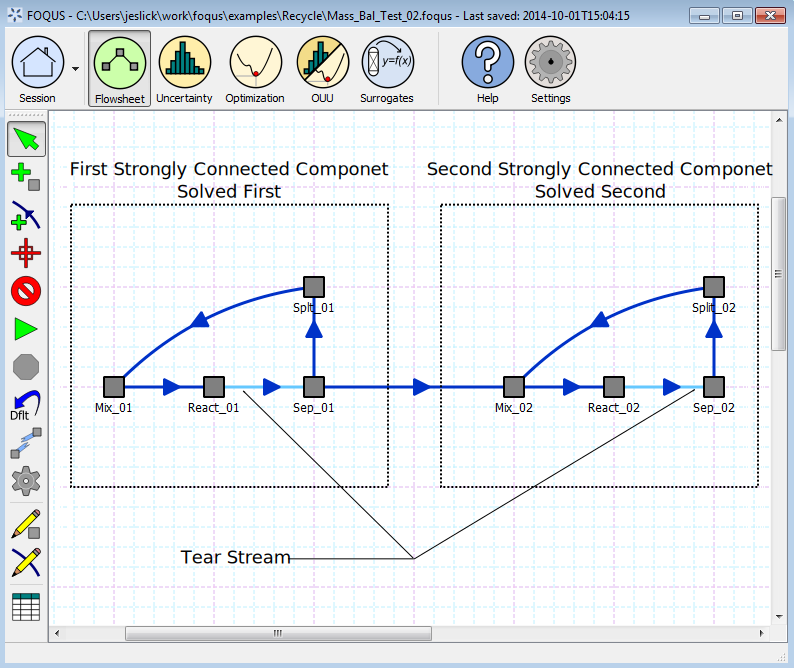
\includegraphics[scale=0.55]{Chapt_flowsheet/figs/recycle}
		\caption{Flowsheet Recycle}
		\label{fig.flowsheet.recycle}
	\end{center}
\end{figure}

\subsection{Flowsheet Editor}
Figure \ref{fig.flowsheet.editor} illustrates the main \bu{Flowsheet Editor} screen and a description of the pieces. The toolbar on the left contains various flowsheet tools.
\begin{figure}[H]
	\begin{center}
		\includegraphics[scale=0.55]{Chapt_flowsheet/figs/flowsheetEdit}
		\caption{Flowsheet Editor}
		\label{fig.flowsheet.editor}
	\end{center}
\end{figure}

The first three buttons are mouse mode buttons.  The current mouse mode is shown by the depressed button. The remaining buttons on the toolbar perform an action. The flowsheet editing toolbar and flowsheet are described in detail below.
\begin{enumerate}
	\item \bu{Selection mode} enables the user to select nodes and edges. Multiple items may be selected by holding down the Shift key. To deselect everything, click an empty area of the flowsheet while not holding the Shift key. Selected items can be moved by dragging them. To move multiple items, hold down the Shift key while dragging. The last item selected becomes the current object to be edited in the \bu{Node} or \bu{Edge Editor}.
	\item \bu{Add node mode} enables the user to add a node by clicking anywhere on the flowsheet. Once a location is clicked, a dialog box opens where the new node name can be entered. If \textbf{\underline{Cancel}} is selected, no node is added. The new node name cannot be ``graph'' and cannot match any existing node name.
	\item \bu{Add edge mode} enables edges to be added by selecting the node that the edge originates from, followed by the node the edge terminates at.
	\item \bu{Center flowsheet in display} centers the display on the flowsheet.
	\item \bu{Delete selected} deletes all selected nodes and edges. If a node is deleted, all edges connecting to that node are also deleted.
	\item \bu{Run a simulation} starts a single simulation run. This is primarily used to test a simulation before running optimization or UQ.
	\item \bu{Stop a simulation} is enabled when a simulation is running and stops any running simulation. The simulation may take several seconds to stop.
	\item \bu{Set inputs to defaults} returns all of the inputs to their default values.
	\item \bu{Determine tear edges} makes it easier to see where initial guesses are needed and makes it possible to edit the tear set before running the flowsheet.  If tear streams are needed but not specified before running a flowsheet, they will be automatically specified, however inputs that will be used for the initial guess will not be known before running.
	\item \bu{Flowsheet solver settings} contains options related to tear solvers.
	\item \bu{Toggle node editor display} displays or hides the \bu{Node Editor}. The user can change the node being edited by selecting from \bu{Name} in the \bu{Node Editor} or selecting it on the flowsheet in selection mode.
	\item \bu{Toggle edge editor display} displays or hides the edge editor. The user can change the edge being edited in the \bu{Edge Editor}, or by selecting it in selection mode.
	\item \bu{Show results from all flowsheet runs} displays the results of all flowsheet runs in a table view. This can be exported to a spreadsheet.
	\item \bu{Node} represents a simulation or calculations.
	\item \bu{Edge} connects simulation data, represents data transfer between two nodes.
\end{enumerate}

\subsection{Node Editor}
The \textbf{\underline{Node Editor}} enables the assignment of simulations to a node, and editing variables. Figure \ref{fig.node.editor.input} shows the Node Editor window with the input variables section of the toolbox displayed.
\begin{figure}[H]
	\begin{center}
		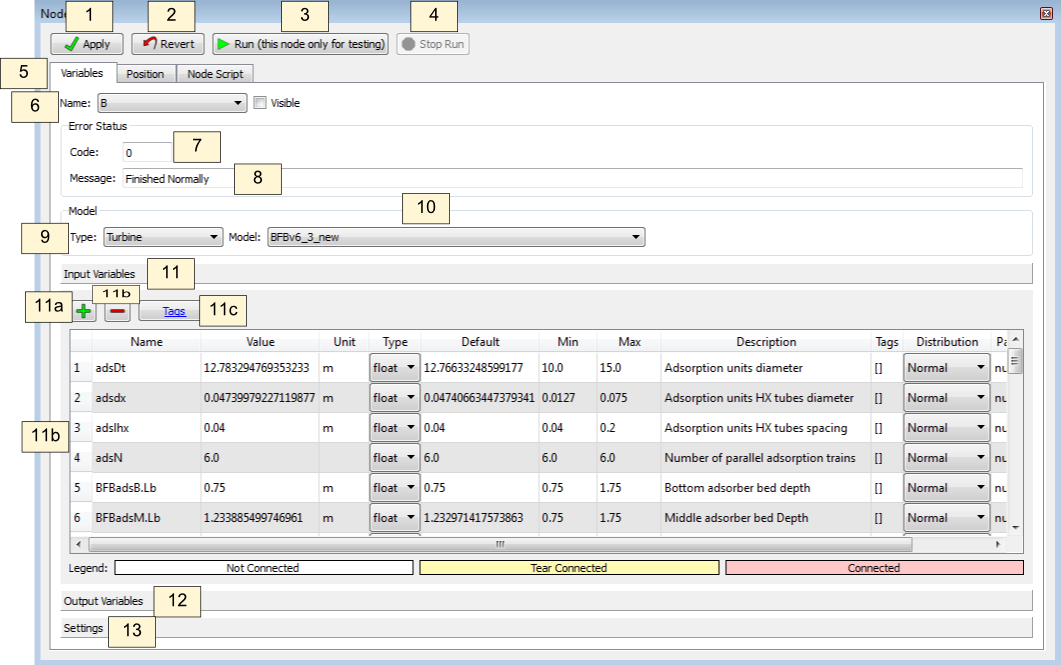
\includegraphics[scale=0.55]{Chapt_flowsheet/figs/nodeEditInput}
		\caption{Node Editor Window}
		\label{fig.node.editor.input}
	\end{center}
\end{figure}

\begin{enumerate}
	\item \bu{Apply} immediately applies any changes made in the \textbf{\underline{Node Editor}}. This is not usually needed. Changes are applied when the current node is changed, the \textbf{\underline{Node Editor}} is closed, or some other action is taken that requires the flowsheet, such as running the flowsheet.
	\item \bu{Revert} sets the node back to the version where the changes were last applied.  This is usually the original state of the node when the editor was opened.
	\item \bu{Run} can be used to run the simulation represented by this node only.  This can be used for testing to make sure the node is properly configured without running the whole flowsheet.
	\item \bu{Stop Run} is active when a simulation is currently running. It stops a single node run or a flowsheet run.
	\item There are three tabs in the \textbf{\underline{Node Editor}}: (1) \bu{Variables} tab, shown in Figure \ref{fig.node.editor.input}, (2) \bu{Position} tab displays the coordinates of the node, and (3) \bu{Node Script} tab enabling the entry of Python code to be executed after the simulation is run.
	\item \bu{Name} displays the name of the node currently being edited. The current node can be changed by selecting from existing nodes in the drop-down menu.
	\item \bu{Code} displays the error status code for the node.
	\item \bu{Message} displays a more detailed description of the error status of the node.
	\item \bu{Type} enables the user to select the type of model to run. The model types are none, Turbine, DMF Lite, DMF Server, or Python Plugin. None allows no model to be assigned to the node; this is useful when the node only executes a script entered directly into FOQUS. Turbine is used to execute Aspen, gPROMS, or Excel simulations. If simulations are stored in either the DMF lite or DMF server, the DMF type models can be used. FOQUS will automatically upload DMF models to Turbine as needed. Python plugins are custom simulations or wrappers written by the user.  Surrogate model methods may also produce Python plugin models.
	\item \bu{Model} enables selection of the models available on Turbine or loaded Python plugins.
	\item \bu{Input Variables} enables viewing and editing the node's input variables. Most of these variables are added automatically when a simulation is selected.
	\begin{enumerate}
		\item \bu{Add variable} enables the addition of an input variable. There are two reasons to add an input: (1) to use a variable to pass information to another simulation (even if the variable is not used in any node calculation, it can receive data from the previous simulation and be passed on to the next simulation) and (2) to use in a node script. For example, a variable could be added that provides output in different units of measure.
		\item \bu{Remove variable} removes variables. If an input variable is removed that originally came from a Turbine simulation, the simulation will run with the default value.
		\item \bu{Tags} displays a tag browser that lists commonly used variable tags.
		\item \bu{Input Variables} table displays information about variables. Most attributes can be edited, except for the \textbf{\underline{Name}} column within the \textbf{\underline{Input Variables}} table. The rows for input variables are color coded depending on whether they are set by an edge from results in another node. White rows are not connected. Yellow rows are set by a tear edge. These variables serve as initial guesses but their value may change once the simulation has run. Red rows are set by an edge that is not a tear edge. The value set for these inputs does not matter and it may change once the simulation has run.
	\end{enumerate}
	\item \bu{Output Variables} is a variable table similar to the \textbf{\underline{Input Variables}} table for node output variables.  This area is displayed by clicking \bu{Output Variables}.
	\item \bu{Settings} displays simulation settings. A description is provided for each setting. The available settings vary depending on simulation.
\end{enumerate}

\subsection{Node Variables}
Variables in the node editor are grouped into two sections, inputs and outputs. The input and output variable tables are accessible as described in the previous section.  The contents of the variable tables are described here.

The columns in the input variable list are:
\begin{itemize}
	\item \bu{Name} is the name of the variable,
	\item \bu{Value} is the current value,
	\item \bu{Unit} is the unit of measure,
	\item \bu{Type} is the data type (float, int, or str),
	\item \bu{Default} is the default value,
	\item \bu{Min} is the minimum value,
	\item \bu{Max} is the maximum value,
	\item \bu{Description} is a description string,
	\item \bu{Tag} is a list of strings that can be used to attach additional information to a variable
	\item \bu{Distribution} is a distribution type,
	\item \bu{Param1} is the first parameter of a parametric distribution the exact meaning depends on the selected distribution, and
	\item \bu{Param2} is the second parameter of a parametric distribution the exact meaning depends on the selected distribution.
\end{itemize}
The minimum and maximum values for are not enforced when running simulations are not enforced.  A value can be given outside the range. Optimization and UQ features make use of these values to set upper and lower bounds on decision variables or sampling. The distribution information is used when setting up sampling for UQ.  In the future, this may also be used for things like optimization under uncertainty.  Integer and string type variables cannot currently be used as optimization decision variables, or sampled with the UQ tool.

The rows of the input variable table are color coded.  Some of the input variables may be set by connections to other nodes.  White rows are variables who's values are not set by a connection.  The variables that are red have values set by a connection, and the value given will be overwritten and does not matter.  The values that are colored yellow are inputs set by a connection that is a tear stream.  The values of these variables serves as an initial guess for solving recycles.

The output variable table is similar to the input table, however it only contains the columns: Name, Value, Unit, Type, Description, and Tags.  The value of the outputs may not correspond to the inputs until the simulation has been run.


\subsection{Node Script}

There are three type of \textbf{\underline{Node Script}} that can be used: (1) \bu{Pre} runs before a node simulation, (2) \bu{Post} runs after a node simulation, and (3) \bu{Total} scripts how a node runs the simulation.

Figure \ref{fig.post.calc} illustrates the \bu{Node Script} tab of the \textbf{\underline{Node Editor}} with calculations for an optimization test problem.

\begin{figure}[H]
	\begin{center}
		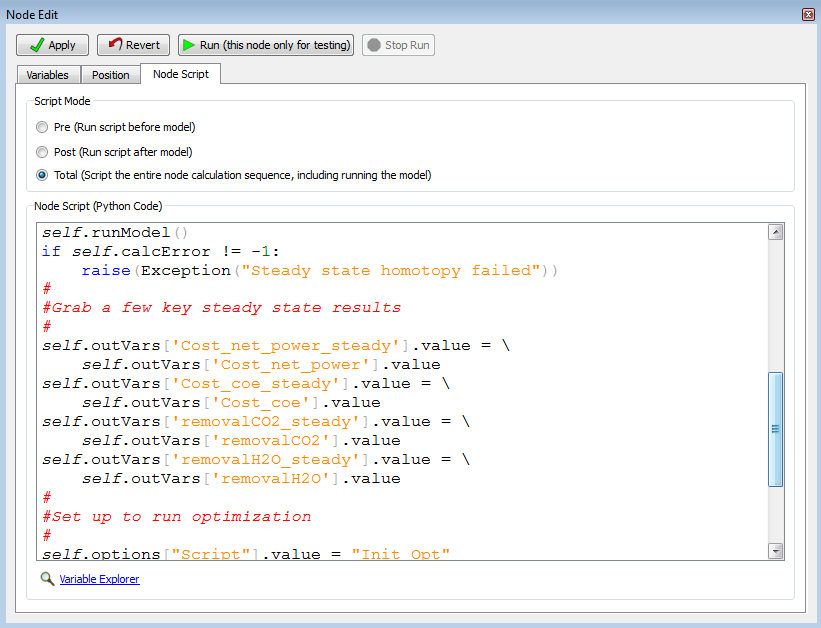
\includegraphics[scale=0.55]{Chapt_flowsheet/figs/postCalc}
		\caption{Node Script Tab}
		\label{fig.post.calc}
	\end{center}
\end{figure}

Node scripts can be any valid Python code. The input and output variables for node scripts are stored in dictionaries x and f. The dictionary keys are the variable names. The f dictionary is used to update the node variables after the calculations are executed.

\subsection{Edge Editor}
The \textbf{\underline{Edge Editor}} is illustrated in Figure \ref{fig.edge.editor}.  The \textbf{\underline{Edge Editor}} can be used to set connections between node variables.

\begin{figure}[H]
	\begin{center}
		\includegraphics[scale=0.55]{Chapt_flowsheet/figs/edgeEdit}
		\caption{Edge Editor}
		\label{fig.edge.editor}
	\end{center}
\end{figure}
\begin{enumerate}
	\item \bu{Index} is the index of the current edge. The current edge can be changed by selecting an index from the drop-down menu, but since the index is not a very meaningful identifier it is usually more convenient to select the edge to edit with the graphical selection tool.
	\item \bu{Origin Node} is the node where an edge starts. This may be edited by selecting a different node from the drop-down menu.
	\item \bu{Destination Node} is the node to which the edge goes.
	\item \bu{Curve} can be a positive or negative number. The greater the magnitude of number, the more curved an edge will appear in the flowsheet. This setting is used to keep edges from overlapping in the flowsheet display.
	\item \bu{Tear} marks this edge as a tear.  Before a simulation is run, if a valid tear set is not specified, FOQUS locates one.
	\item \bu{Active} specifies whether the edge is active or not. This allows connections to be temporarily disabled.
	\item \bu{Variable Connections} table displays which variables are connected.  Inputs or outputs in the origin node can be connected to inputs in the destination node.
	\item \bu{Add connection} adds a new connection.
	\item \bu{Remove connection} deletes the selected connections.
	\item \bu{Auto} automatically connects variables having the same name. For example, in connecting a simulation to a spreadsheet to calculate costs there are a large number of variables for which it makes sense that the variables have the same name in the simulation and spreadsheet. \bu{Auto} should be used with great care. Connecting variables with the same name is often not what is wanted. For example two simulations may have a variable named FlowAIn; however, it is very unlikely that they should be connected. It is more likely FlowAOut should be connected to FlowAIn.
\end{enumerate}

